\documentclass[/home/greg/Thesis/main/main.tex]{subfiles}

%\title{Neutron star mechanics in the observers inertial frame}
%\author{}

\begin{document}
\graphicspath{{/home/greg/Neutron_star_modelling/BeamwidthCalculation/img/}}
\subsubsection{Missing the other pole}
We now discuss an issue arising in the precessional interpretation of B1828-11
and other pulsars which demonstrate a double-peaked spin-down rate. The precessional
interpretation asserts that the two harmonics naturally arise in pulsars
for which $\chi \approx \pi/2$. In such circumstances the precessional wobble
    causes the magnetic dipole to wander of the rotation equator. This is a maximum
    in the torque and as such coincides with a minimum of the spin-down rate.

If such an interpretation is to be believed, then we should expect to see an 
inter pulse corresponding to the other pole. To illustrate this consider an
observer in the northern hemisphere of a pulsar undergoing free precession.
We denote the fixed angular momentum vector of the star by $\J$ and
set the spin-vector to be at a small angle $\theta$ to $\J$. The
motion of the EM dipole can be understood as tracing a cone about $\J$
of half-angle $\Theta$ at the fast rotation frequency; precession then causes
a slow modulation of the dipoles polar angle $\Theta$ by an amount $\Delta\Theta$.  
Since the observer will only observe a pulse when the dipole cuts the plane
containing the observer and $\J$, we can illustrate the picture using
the diagram in Fig.~\ref{fig: dipole close to 90}. On the long precession time
scale, the observer sees $\m$ oscillate in the range $\Delta \Theta$ depicted
in the figure.

\begin{figure}[htb]
\centering
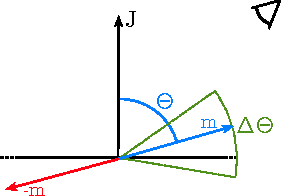
\includegraphics[width=0.5\textwidth]{img/MissingTheOtherPole}
\caption{Illustration of the observer, the angular momentum vector $\J$ and
the two sides of the magnetic dipole $\m$ as it cuts the plane containing
the observer and angular momentum vector.}
\label{fig: dipole close to 90}
\end{figure}

In this image we have presented a rather special case, let us first review the
more general case:
\begin{itemize}

\item With $\Theta < \pi/2$, then the angular distance between the blue pole of
the beam and the observer is always larger than that between the red pole and
the observer (at $\pi$ out of phase from this picture when the red pole is on
the observer side of $\J$ and hence beaming towards the observer). In such a
case the observer, if they see any pulses at all, will always see the blue pole
as the most intense beam. If the beam is sufficiently strong and or $\Theta
\approx \pi/2$ (but still smaller), then the observer may also observe the red
pole as an inter-pulse $\pi$ out of phase from the blue pole.

\item If $\Theta$ ranges over $\pi/2$ as shown in Fig.~\ref{fig: dipole close
to 90} then the blue pole is not always the closest angular distance to the
observer: during the period for which $\Theta>\pi/2$, the red pole will have a
closer angular separation to the observer when beaming towards the observer. Now,
provided the intensity of both beams are approximately equivalent, the observer
must see the `inter-pulse' stronger than the main beam.
\end{itemize}

For B1828-11 several publications have estimated best-fit parameters which would
cause the beam to wander of the rotational equator, yet no inter-pulse or any
evidence of a second beam is observed. One possible explanation is that the
red-pole is misaligned in a polar-sense from the blue-pole. In
figure~\ref{fig: dipole close to 90 missaligned} we illustrate such a case labelling
the angle of misalignment by $\lambda$. Pulsars are observed with this geometry
[need to fill in typical ranges]. 


\begin{figure}[htb]
\centering
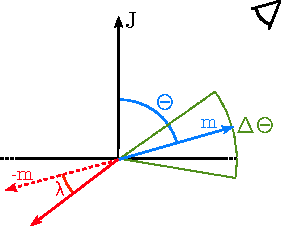
\includegraphics[width=0.5\textwidth]{img/MissingTheOtherPoleMissaligned}
\caption{Repeat of Fig.~\ref{fig: dipole close to 90 missaligned} with the addition
of a misaligned red pole.}
\label{fig: dipole close to 90 missaligned}
\end{figure}

The absence of any observed inter-pulse in B1828-11 can then be explained if
\begin{equation}
\lambda > \langle\Theta\rangle + \Theta/2
\end{equation}
which would prevent the red pole from rising into the northern hemisphere and
becoming as bright as the observed pulse. Of course, we could also postulate that
the red pole is a weaker beam..
\biblio
\end{document}

